\documentclass[instructions]{uqthesis}
%\documentclass[final]{uqthesis} 


%*************************************
% FOR YOUR FINAL THESIS
%*************************************

%IMPORTANT! 
%The default document class (above - line 1 & 2) for the template is \documentclass[instructions]{uqthesis} - this document class will show instructional material and examples relevant to the preliminary material in the compiled PDF preview. THESE INSTRUCTIONS ARE FOR YOUR REFERENCE ONLY AND ARE NOT TO BE INCLUDED IN YOUR FINAL THESIS! 

%To turn off these instructions in your final thesis you MUST use the document class \documentclass[final]{uqthesis} 
%To activate the final thesis document class you must UN-COMMENT THIS DOCUMENT CLASS (remove the % from the start of line 2) and comment out the instructional document class on line 1 (add % to the start of line 1). 

%*************************************
% Introduction to template
%*************************************
%This is The University of Queensland Graduate School Official LaTeX Thesis template.

%Be sure to observe the content of comments within the source code, these are prefaced with a percentage symbol.
%Most important instructions have been CAPITALISED.
%To uncomment an inactive command (if required) remove the % from in front of the command.

%Please see the README for more information.

%This file loads the necessary packages, sets the page styles, and defines required macros.
%Edit this if you are comfortable with LaTeX.

%Other tweaks can be made in uqthesis.cls, but change these at your own risk!

%See README for version.

%You must have the memoir class installed.

\input{LaTexPackages.tex}

\newif\ifnotes
% Bib commands
\newcommand{\nat}{Nature}
\newcommand{\apjl}{The Astrophysical Journal}
\newcommand{\apj}{The Astrophysical Journal}
\newcommand{\ssr}{Space Science Reviews}
\newcommand{\mnras}{Monthly Notices of the Royal Astronomical Society}
\newcommand{\physrep}{Physics Reports}
\newcommand{\aap}{Astronomy \& Astrophysics}
\newcommand{\araa}{Annual Review of Astronomy and Astrophysics}
\newcommand{\aapr}{The Astronomy and Astrophysics Review}
\newcommand{\na}{New Astronomy}
\newcommand{\pasj}{Publications of the Astronomical Society of Japan}
% Generic
\newcommand{\Msun}{M$_\odot$}
\newcommand{\stickynote}[1]{
  \ifnotes
    \marginnote{\color{red}\footnotesize\textbf{#1}}
  \fi
}
% Set header style
\fancyhead{}
\fancyhead[RE]{\leftmark}   % Even pages
\fancyhead[LO]{\rightmark}  % Odd pages
\fancyfoot[C]{\thepage}
\renewcommand{\footrulewidth}{0pt}
\renewcommand{\headrulewidth}{0pt}

% Toggle self notes
\notestrue

% ***************************************************
% Title page
% ***************************************************
%***THESIS TITLE***
%Use Sentence Case (capitalise only the first word and proper nouns).
\title{A fantastic title about minihalos that somehow grips a viewers attention for over 100 pages of detail}

%***YOUR NAME***
%Do not include initials or middle names. Do not include your supervisor(s)' name(s).
\author{Benjamin Colquhoun}

%***YEAR OF SUBMISSION***
\date{2026}

\school{Te Herenga Waka - Victoria University of Wellington}

\begin{document}
\frontmatter
% Assemble title page
\maketitle

\clearpage

% ***************************************************
% Preface
%****************************************************
\section*{Abstract}
\phantomsection
\addcontentsline{toc}{chapter}{Abstract}

\normalfont
%Open abstract.tex to edit
% ***************************************************
% Abstract
% ***************************************************
% TO PRODUCE A STAND-ALONE PDF OF YOUR ABSTRACT, uncomment this section and the \end{document} at the end of the file by removing the % from the start of each line.

%\documentclass[12pt, a4paper]{memoir}

%\input{LaTexPackages.tex}

%\begin{document}

%\begin{center}
	%\textbf{\large Your title goes here}

	%\textbf{Abstract}

	%Your Name, The University of Queensland, 20??
%\end{center}

% ********* Enter your text below this line: ********
Diffuse radio sources have been found within the cool cores of a growing number of relaxed galaxy clusters. These faint `minihalos' are a result of synchrotron-emitting, highly relativistic electrons. With extents over several hundred kiloparsec, they are far beyond the expected extent of a single source of relativistic electrons. The processes of \textit{in-situ} turbulent reacceleration and hadronic production have been proposed to explain this phenomenon. Spectral steepening is expected at high radio frequencies for the reacceleration scenario, however, the majority of previous studies have been performed at lower radio frequencies (144 MHz to 1.4 GHz) where this is difficult to detect.

To investigate potential steepening, in this thesis I calibrate and image Very Large Array radio interferometer observations at 10 GHz of 12 clusters hosting minihalos. This represents the first steps towards a high frequency survey of minihalos. Source-subtracted measurements of minihalo flux are performed for four clusters, enabling comparison with prior observations at lower frequencies. Steepening was not observed for three clusters, RXJ1720+2638 ($\alpha=1.1\pm0.05$), RXCJ1115+0129 ($\alpha=1.03\pm0.18$), and RXJ2129+0005 ($\alpha=1.18\pm0.09$). This suggests a hadronic origin for these minihalos. One cluster, A478 ($\alpha=2.02\pm0.10$), exhibits tentative evidence of steepening, however, more research is required to ensure this is not from instrumental effects. The remainder of the sample requires more extensive analysis. Challenges encountered during the calibration and imaging are discussed, and recommendations for future analysis of high frequency minihalo studies are presented. 
% ***************************************************

%\end{document}

\clearpage
% ***************************************************
% \section*{Declaration by author}
% %DO NOT EDIT.
% \input{./Authordeclaration.tex}

% \clearpage
% %YOU MUST EDIT THIS DOCUMENT.
\pagestyle{fancy}
% ***************************************************
% PRELIMINARY PAGES
% ***************************************************
% The instructions contained within this part of the thesis template need to be suppressed from the final thesis. There are instructions on how to do this in the MainThesis.tex file.

% To ensure your work is not suppressed with the instructions please add your text only where instructed.

%***Acknowledgements***
\clearpage
\section*{Acknowledgments}
\phantomsection
\addcontentsline{toc}{chapter}{Acknowledgements}

\begin{instructional}
    \noindent
    People who helped me during my Thesis: Yvette, CASA people, sibling. 
\end{instructional}


% ***************************************************

%***Table of Contents***
%These generate the table of contents, list of figures, and list of tables from items tagged with a \label{} command.
\clearpage
\tableofcontents
\newpage

%***End of front matter***

% ***************************************************
% Thesis Content
%****************************************************
\mainmatter
\pagestyle{fancy}

%Each chapter is a separate .tex file. Use \input to load them here, as demonstrated below for Chapter 1 and Chapter 2.
%We recommend keeping each in a separate subfolder, with its accompanying figures, etc. This is how the template is currently structured.
%If you wish to divide your thesis into parts (each containing multiple chapters), us the \part{} command.

%CHAPTER 1
\chapter[Introduction]{Introduction}
\label{Chap:Intro}

% ***************************************************
% Introduction
% ***************************************************

\section{Galaxy Clusters}
\begin{itemize}
    \item What is a Galaxy Cluster (grav bound galaxies, in a bunch of hot gas)
    \item Generic information about galaxy clusters (yay statistics)
    \item Fun facts about galaxy clusters
\end{itemize}

\section{Observational work with Galaxy Clusters}
\begin{itemize}
    \item Well, we can't just go there so we get to look at them really closely.
    \item How do we get data about clusters
    \item In increasing wave length, Optical, X-ray, Radio, Gamma. 
    \item Some telescope + research that we can do with each of these.
\end{itemize}

\section{Radio Emission}
\begin{itemize}
    \item This is what we are interested in, can gain information about clusters from this.
    \item Link synchrotron emission to the electron / gas properies of the cluster and how radio emission can inform us of what the cluster is doing.
    \item Common sources of relativistic electrons are the AGNs, lose energy over time. 
    \item Structures larger than the lifetime of these jets, more diffuse (Halos).
\end{itemize}

\subsection{Giant Radio Halos}
\begin{itemize}
    \item These are of similar extent to the cluster gas. 
    \item They 
\end{itemize}

\subsection{Minihalos}
'\begin{itemize}
    \item What is a minihalo (diffuse radio emission in the core of a cluster.)
    \item Actually they are somewhat common. 
    \item Talk about some previous works on minihalos
    \item Difficulty in distinguishing between production mechanisms.
\end{itemize}

\section{Our goals}
\begin{itemize}
    \item We want to be able to measure minihalo flux for this subset of minihalos at high radio frequencies so that we can investigate if steepening is occuring.
\end{itemize}

\chapter[Observations]{Observations}
This chapter would be about radio interferometry, how it works to some extent and the data that is retrieved from it. How to calibrate the data etc.

\section{What is an interferometer}
\begin{itemize}
    \item Limits of dish size in resolution, causes us to explore different ideas.
    \item How does an interferometer work.
    \item Bunch of dishes being interfered, delay to tune positioning, uv plane to determine coverage.
    \item From all of this we retrieve amp + phase measurements.
\end{itemize}

\section{Our observations}
\begin{itemize}
    \item We are using VLA data in X-band, what does this mean and what are the specs for the VLA.
    \item These observations are of list minihalos and this setup, observation proposal.
    \item Original source of these minihalos is the G14 paper (among others).
    \item Table of minihalos + observing setup.
\end{itemize}


\chapter[Calibration]{Calibration}
This would be how to calibrate and the calibration results for the datasets, plus any special considerations we took.

\section{How to calibrate a dataset}
\begin{itemize}
    \item We have the VLA calibration pipeline to remove stress from our lives.
    \item We have a non-neglible amount of RFI to add stress to our lives. 
    \item A variety of steps but first pain, what is RFI and what does it cause.
\end{itemize}

\section{Flagging data}
\begin{itemize}
    \item Initial testing showed that the pipeline flagging steps didn't work well for our data.
    \item AOFLAGGER worked much better and has a mostly out-of-box VLA script.
    \item How does AOFLAGGER work
    \item Integrating into a pipeline step to still use the pipeline
\end{itemize}

\section{Calibration pipeline}
\begin{itemize}
    \item Work through each calibration step explaining what it does and why it is important. 
    \item Final preparation for imaging is averaging down to further reduce noise.
    \item Notes about general trends from the calibration, with RFI in 10-12 GHz D config being bad, much of it being flagged.
\end{itemize}

\section{Special mentions}
\begin{itemize}
    \item Either here or during following imaging section talk about the 2-3 datasets we processed slightly differently due to bad fits.
    \item Describe the fitting process for the custom bandpass.
\end{itemize}

\chapter[Analysis Tools]{Analysis Tools}
This chapter starts with an overview on imaging and how that is performed. Then we talk a bit about how we actually want to measure the flux of the minihalos.
Could combine with actual results.

\section{Imaging}
\begin{itemize}
    \item When we make a raw image from the data, we still have a lot of artefacts from the point spread function, which comes from the beam.
    \item This means we need a more advanced imaging process to remove this to get a clean image. Implemented in a few different ways, we choose tclean in CASA.
    \item Tclean works by modelling the PSF, creating an empty model, find brightest point in residuals, model that as real, subtract model from residuals, repeat 20K times.
    \item This works mostly well, but we can improve results using self calibration.
\end{itemize}

\subsection{Self calibration}
\begin{itemize}
    \item The phase calibration is the most iffy part for the main calibration, so we can make a test image and check the model seems reasonable.
    \item Then use that model to make small phase corrections to our dataset. Then repeat that a few times and these corrections should converge since it is circular.
    \item This is the final calibration steps that we do, phase corrections 20 degrees $\rightarrow$ 1 degree after a few rounds. 
\end{itemize}

\subsection{Final cleaning}
\begin{itemize}
    \item Between self calibrations this we also check the datasets and do some final manual cleaning.
    \item Clipping the datasets to a sensible amp range, removing spikes, SPWs where there is small amounts of data left.
    \item Overview of the \texttt{assess\_spw} function used for this.
\end{itemize}

\section{Final datasets}
\begin{itemize}
    \item Could have a table here talking about each minihalo, how much data is remaining, spws that are flagged out, some sort of visual. 
    \item Maybe bar graph of spws, line or point graph for minihalo C/D (either total or differentiated by style) normalised to [0, 1]
\end{itemize}

\section{Calibration Error}
\begin{itemize}
    \item Calibration error exists, and sources can vary in their flux amount.
    \item We can try and constrain the error and variance by comparing the secondary calibrator models for D config and the point source fluxes for the images.
    \item Fluxes for secondaries can vary a lot over a year (100\%?) maybe, but lower per month. Can then compare to differences in sources in the image.
    \item If a trend is observed, likely calibration error. If no trend or close models, constrain calibration error and can see the variance in AGN etc.
    \item Can retrieve the point source flux by cutting out diffuse sources (uvrange) and by masking to a tight border.
\end{itemize}

\section{Calculating the minihalo flux}
\begin{itemize}
    \item We can do this in a variety of ways, but we don't want the AGN contamination so we should subtract this out.
    \item Do this per dataset to account for variation over time, incorrect subtractions can result in negative bowls in emission, or remaining flux.
    \item Other problematic sources are dealt with the same way.
    \item Image the subtracted data and then we create a contour for significant emission (3 sigma) from the residual RMS.
    \item Calculate total flux in the region.
    \item Then we calculate the error using this formula from G14 modified for the AGN error since we think its lower.
\end{itemize}

\chapter[Results]{Results}
\begin{itemize}
    \item Sections for each minihalo with a brief explanation of imaging process, custom things we had to do to get results.
    \item Number of self calibration, sources subtracted, difficulties in imaging certain aspects.
    \item Discussion on the calibration error and variance in the observed point sources.
    \item Includes an image of the uvrange data showing point sources, image of the minihalo with contours, and anything else we desire.
    \item Includes discussion compared to previous results or measured values (likely G14) and any caveats or concerns.
\end{itemize}

%CHAPTER 2
\chapter[Minihalos]{Minihalos}
\label{Chap:Background}

Since the first discoveries of diffuse radio emission, much research has been devoted towards understanding the mechanisms behind the production of synchrotron electrons. These electrons are also known as `cosmic ray' (CR) electrons or non-thermal electrons to differentiate them from the thermal electrons of the ICM. In the case of CR electrons within the thin plasma of the ICM, we make the standard assumption that the population of CR electrons is homogeneous and isotropic and follows a power-law energy distribution $n(E) \propto E^{-\delta}$. From this we then predict the following basic observables (see \citet{vanWeeren2019}, \citet{Ferreti2012} and references within). \stickynote{Add graph of spectral shapes?}

\begin{enumerate}
    \item The synchrotron emissivity is dependent on the number density of the CR electrons and the strength of the magnetic field. As such, the emissivity also follows a power-law $S(\nu) \propto \nu^{-\alpha}$ which is related to $\delta$ by $\alpha = (\delta - 1)/2$. Typical minihalo spectral indices are steep with $\alpha > 1$.
    \item Over time the emitting particles lose energy, which changes the particle energy distribution and therefore, the emitted radio spectrum. This appears as a steepening or curved spectrum, rather than a flat power-law. The break frequency at which this occurs is related to the time of acceleration. This means that radio events that have stopped will show an aged spectrum with a characteristic break, such as radio relics, while ongoing events are continually injecting new particles and don't feature the same steepening due to age. 
    \item Radiation from CR electrons passing through a uniform magnetic field is linearly polarised. Non-uniform and disordered fields reduce the linear polarisation. 
\end{enumerate} 

\section{Production mechanisms}

The 

\subsection{Turbulent re-acceleration}

\label{sec:BG_reacceleration}
\begin{itemize}
    \item What is the process here.
    \item How manifest spectrally.
    \item How manifest spatially.
\end{itemize}

\subsection{Hadronic Production}
\label{sec:BG_hadronic}
\begin{itemize}
    \item What is the process for hadronic production
    \item How does this manifest spectrally and evolve. What should we expect observationally here based on simulation work.
    \item How does this manifest spatially and evolve, what should we see observationally.
\end{itemize}



\subsection{Large Radio Halos}
\begin{itemize}
    \item Use similar physics but much larger scale. 
    \item Some basics things about previous research in differentiating production. 
    \item Gamma ray non-detection.
    \item General consensus is that its re-acceleration.
\end{itemize}

\subsection{Minihalos}
\begin{itemize}
    \item These are much smaller, so therefore much harder to observe. Difference to large radio halos.
    \item Similarities between host clusters (CC), general properties of spectral index etc.
\end{itemize}









\subsection{Previous minihalo studies}
\begin{itemize}
    \item Generally look at lower frequencies, or a singular study for a particular minihalo.
    \item Want to look at more minihalos in a more holistic manner. 
    \item Some findings from previous papers e.g. RXJ1720, MS1455+2232 in basic detail. (more detail on the per-halo discussion).
\end{itemize}


%CHAPTER 3
\chapter[Calibration]{Calibration and Imaging}
\label{Chap:Calibration}
This would be how to calibrate and the calibration results for the datasets, plus any special considerations we took.

\section{Our observations}
\begin{itemize}
    \item We are using VLA data in X-band, what does this mean and what are the specs for the VLA.
    \item These observations are of list minihalos and this setup, observation proposal.
    \item Original source of these minihalos is the G14 paper (among others).
    \item Table of minihalos + observing setup.
\end{itemize}

\section{How to calibrate a dataset}
\begin{itemize}
    \item We have the VLA calibration pipeline to remove stress from our lives.
    \item We have a non-neglible amount of RFI to add stress to our lives. 
    \item A variety of steps but first pain, what is RFI and what does it cause.
\end{itemize}

\section{Flagging data}
\begin{itemize}
    \item Initial testing showed that the pipeline flagging steps didn't work well for our data.
    \item AOFLAGGER worked much better and has a mostly out-of-box VLA script.
    \item How does AOFLAGGER work
    \item Integrating into a pipeline step to still use the pipeline
\end{itemize}

\section{Calibration pipeline}
\begin{itemize}
    \item Work through each calibration step explaining what it does and why it is important. 
    \item Final preparation for imaging is averaging down to further reduce noise.
    \item Notes about general trends from the calibration, with RFI in 10-12 GHz D config being bad, much of it being flagged.
\end{itemize}

\section{Special mentions}
\begin{itemize}
    \item Either here or during following imaging section talk about the 2-3 datasets we processed slightly differently due to bad fits.
    \item Describe the fitting process for the custom bandpass.
\end{itemize}

\section{Imaging}
\begin{itemize}
    \item When we make a raw image from the data, we still have a lot of artefacts from the point spread function, which comes from the beam.
    \item This means we need a more advanced imaging process to remove this to get a clean image. Implemented in a few different ways, we choose tclean in CASA.
    \item Tclean works by modelling the PSF, creating an empty model, find brightest point in residuals, model that as real, subtract model from residuals, repeat 20K times.
    \item This works mostly well, but we can improve results using self calibration.
\end{itemize}

\subsection{Self calibration}
\begin{itemize}
    \item The phase calibration is the most iffy part for the main calibration, so we can make a test image and check the model seems reasonable.
    \item Then use that model to make small phase corrections to our dataset. Then repeat that a few times and these corrections should converge since it is circular.
    \item This is the final calibration steps that we do, phase corrections 20 degrees $\rightarrow$ 1 degree after a few rounds. 
\end{itemize}

\subsection{Final cleaning}
\begin{itemize}
    \item Between self calibrations this we also check the datasets and do some final manual cleaning.
    \item Clipping the datasets to a sensible amp range, removing spikes, SPWs where there is small amounts of data left.
    \item Overview of the \texttt{assess\_spw} function used for this.
\end{itemize}


%CHAPTER 4
\chapter[Analysis Tools]{How to Analysis}
This chapter starts with an overview on imaging and how that is performed. Then we talk a bit about how we actually want to measure the flux of the minihalos.
Could combine with actual results.

\section{Final datasets}
\begin{itemize}
    \item Could have a table here talking about each minihalo, how much data is remaining, spws that are flagged out, some sort of visual. 
    \item Maybe bar graph of spws, line or point graph for minihalo C/D (either total or differentiated by style) normalised to [0, 1]
\end{itemize}

\section{Calibration Error}
\begin{itemize}
    \item Calibration error exists, and sources can vary in their flux amount.
    \item We can try and constrain the error and variance by comparing the secondary calibrator models for D config and the point source fluxes for the images.
    \item Fluxes for secondaries can vary a lot over a year (100\%?) maybe, but lower per month. Can then compare to differences in sources in the image.
    \item If a trend is observed, likely calibration error. If no trend or close models, constrain calibration error and can see the variance in AGN etc.
    \item Can retrieve the point source flux by cutting out diffuse sources (uvrange) and by masking to a tight border.
\end{itemize}

\section{Calculating the minihalo flux}
\begin{itemize}
    \item We can do this in a variety of ways, but we don't want the AGN contamination so we should subtract this out.
    \item Do this per dataset to account for variation over time, incorrect subtractions can result in negative bowls in emission, or remaining flux.
    \item Other problematic sources are dealt with the same way.
    \item Image the subtracted data and then we create a contour for significant emission (3 sigma) from the residual RMS.
    \item Calculate total flux in the region.
    \item Then we calculate the error using this formula from G14 modified for the AGN error since we think its lower.
\end{itemize}



%CHAPTER 4
\chapter[Results]{Results}
\label{Chap:Results}

\section{RXJ1720+2638}
\label{sec:rxj1720+2638}
RXJ1720+2638 (also known as RXJ1720.1+2638) is a cool core galaxy cluster at $z = 0.160$ \citep{Owers2011}. Early observations detected the presence of two cold fronts, an edge to the southeast and a plateau to the northwest \citep{Mazzotta2001}. This suggested the presence of a core dense cold gas cloud ($T \approx 4$ keV) embedded in the outer diffuse and hot ICM ($T\approx10$ keV), with the cold fronts likely arising via a minor merger. Weak gravitational lensing studies \citep{Okabe2010} and galaxy density mapping \citep{Owers2011} revealed the presence of a substructure $\sim550$ kpc north of the cluster core. \citet{Owers2011} suggest that a northward passage of this structure passing the core to the east, providing the perturbations to the core and inducing large scale gas sloshing. RXJ1720+2638 was one of the first two clusters where cold fronts and minihalos were found to have a spatial correlation, with minihalo emission bounded by the cold fronts of the ICM \citep{Mazotta2008}. 

A detailed spectral study was performed by \citet{Giacintucci2014a}, which analysed observations at six frequencies from 317 MHz to 8.4 GHz taken by the GMRT and VLA. To perform accurate comparison between these frequencies, the baselines range was limited to 1--50 k$\lambda$, to enforce a unified sampling of the uv plane. to This noted three primary sources of minihalo emission in the core region, the central radio galaxy (BCG, single power-law $\alpha = 0.87\pm0.03$), a head-tail radio galaxy to the northeast with the tail to the south ($\alpha = 1.05\pm0.04$, steepening down the tail), and the minihalo emission. The BCG was noted to be unresolved with no jets or lobes detected at scales $>1.4$ kpc. Higher angular resolution observations by the extended Multi-Element Radio Linked Interferometer Network (e-MERLIN) at 4.76 GHz found the BCG to exhibit sub-kpc jets \citep{Perrott2023}. The jets extend 0.8 kpc to the east and west, though uncertainty in the recovered flux may indicate further undetected extent. \citet{Giacintucci2014a} separate the emission into a 160 kpc central region and tail region extending 200 kpc to the south. These were found to have spectral indices of $\alpha_c = 1.0\pm0.1$ and $\alpha_t = 1.5\pm0.1$, respectively. The core region exhibits a relatively flat spectral index across the extent, while spectral steepening is observed along the tail. LOFAR images at 144 MHz support the flat spectral index in the core, with steepening across the cold fronts \citet{Savini2019}. The spectral index for the core is consistent to 4.86 GHz, however, the 8.44 GHz measurement was lower than predicted by the single power-law. Although this indicated possible steepening, the 4.86 GHz and 8.44 GHz observations had much poorer uv sampling, which may have caused flux losses from the filtering of large-scale emission. \citet{Perrott2021} perform a high-frequency measurement of the central region of the minihalo was made at 15.5 GHz, using the Arcminute Microkelvin Imager (AMI). They construct a model of the minihalo in the uv plane to account for the spatial filtering, finding the single power-law $\alpha = 1.0$ is consistent to 15.5 GHz.

\subsection{10 GHz observation}
In processing the observations for imaging, two contaminating sources were identified prior to minihalo flux estimation. This included the BCG within the minihalo emission and a variable AGN to the southwest. These were modelled individually per dataset with a uvcut of 15 k$\lambda$ and subtracted. The head-tail source was sufficiently cleaned and tail emission isolated from that of the minihalo. A balance of beam sensitivity and PSF suppression was obtained using a \texttt{robust} of 1. Scales were set to $[0, 4, 8, 16, 32]$ with a \texttt{smalscalebias} of $-0.5$. \citet{Giacintucci2014a} supply details of the masking region, including the separation of centre and tail regions. This allowed a reproduction of these regions for analysis and accurate comparison to previous studies.\stickynote{I also have a 1--50 klambda image} 

The total minihalo flux was measured as $8.72\pm0.44$ mJy, with the majority $7.76\pm0.39$ mJy attributed to the central region and only $0.96\pm0.08$ mJy from the tail. The measured flux densities for relevant sources and regions are provided in Table \ref{tab:rxj1720+2638_flux}. The 10 GHz image is shown in Figure \ref{fig:rxj1720+2638_image}. The spectral index is fit for the total flux, centre, tail, and BCG using values measured from \citet{Giacintucci2014a} (excluding 8.46 GHz) and shown in Figure \ref{fig:rxj1720+2638_seds}. The spectral index of the central minihalo region was $\alpha_c = 1.07\pm0.06$, with a steeper tail region of $1.26\pm0.06$. The central results agree well with the previous result, with the tail found to be slightly flatter on average.

The BCG was measured to vary $\sim\!$20\% over one year (between C and D-configuration runs) and $\sim\!$10\% over one month (subsequent D-configurations). This degree of variation may suggest a systematic calibration error between the D-configuration observations. A systematic offset of $0.7$\% was observed in the flux density models of the secondary calibrator for these observations, other point sources in the image were measured and no systematic offsets were observed. Because of this, and the presence active jets from the BCG, the variation is likely real. 

\begin{table}[h]
    \centering
    \begin{tabular}{l|ccccc}
        \toprule
        Source & Minihalo & Minihalo (Centre) & Minihalo (Tail) & BCG \\ 
        \midrule
        Flux (mJy) & $8.77\pm0.44$ & $7.76\pm0.39$ & $0.96\pm0.08$ & $1.27\pm0.2$\\
        \bottomrule
    \end{tabular}
    \caption{Flux density obtained for sources in RXJ1720+2638 at 10 GHz. The value for the BCG is given as the average of the observed fluxes, with error corresponding to the maximum and minimum obtained.}
    \label{tab:rxj1720+2638_flux}
\end{table}

\begin{figure}
    \centering
    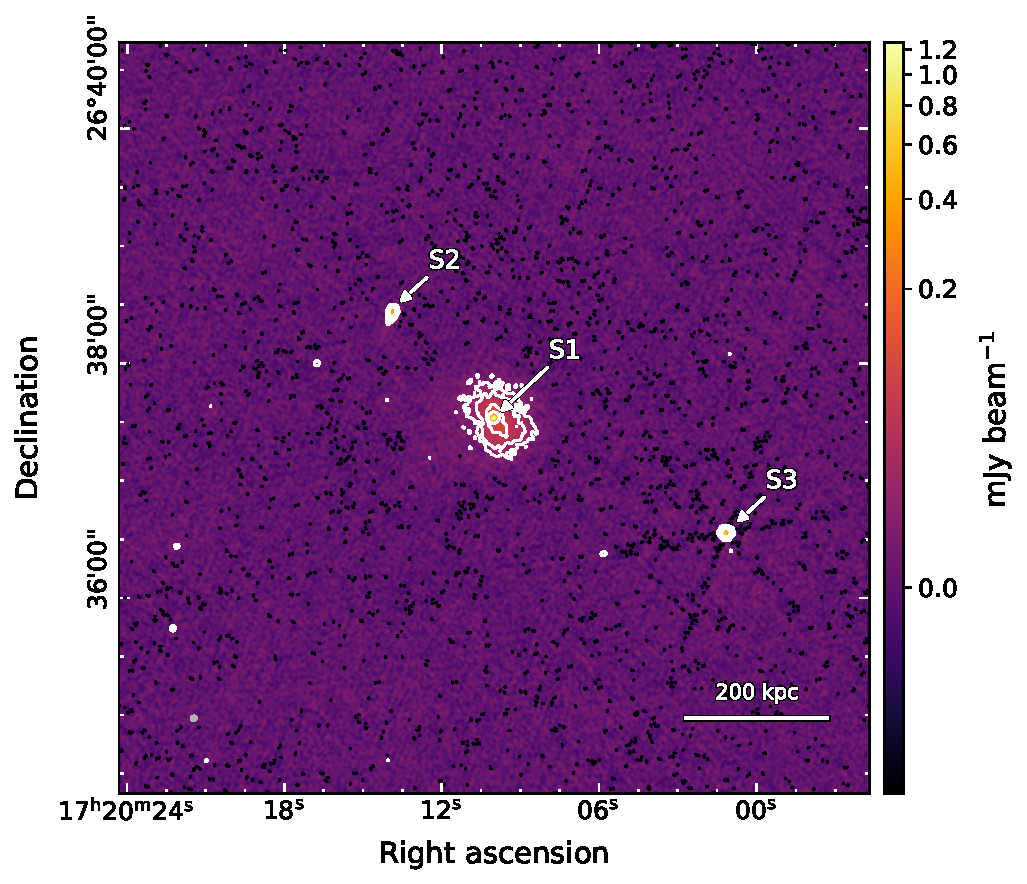
\includegraphics[width=0.85\textwidth]{Chapter5/vla_images/rxj1720.pdf}
    \caption{RXJ1720+2638. Point source subtracted 10 GHz observation with restoring beam $3.52"\times3.17"$ at position angle -34\textdegree{} and noise $1\sigma = 3.12$ $\mu$Jy beam$^{-1}$. Contour levels (white) are spaced in factors of two starting from 3$\sigma$. The masks used for flux estimation is shown in red, marking the centre (solid) and tail (dotted) regions. The green cross marks the location of the subtracted BCG.}
    \label{fig:rxj1720+2638_image}
\end{figure}

\begin{figure}
    \centering
    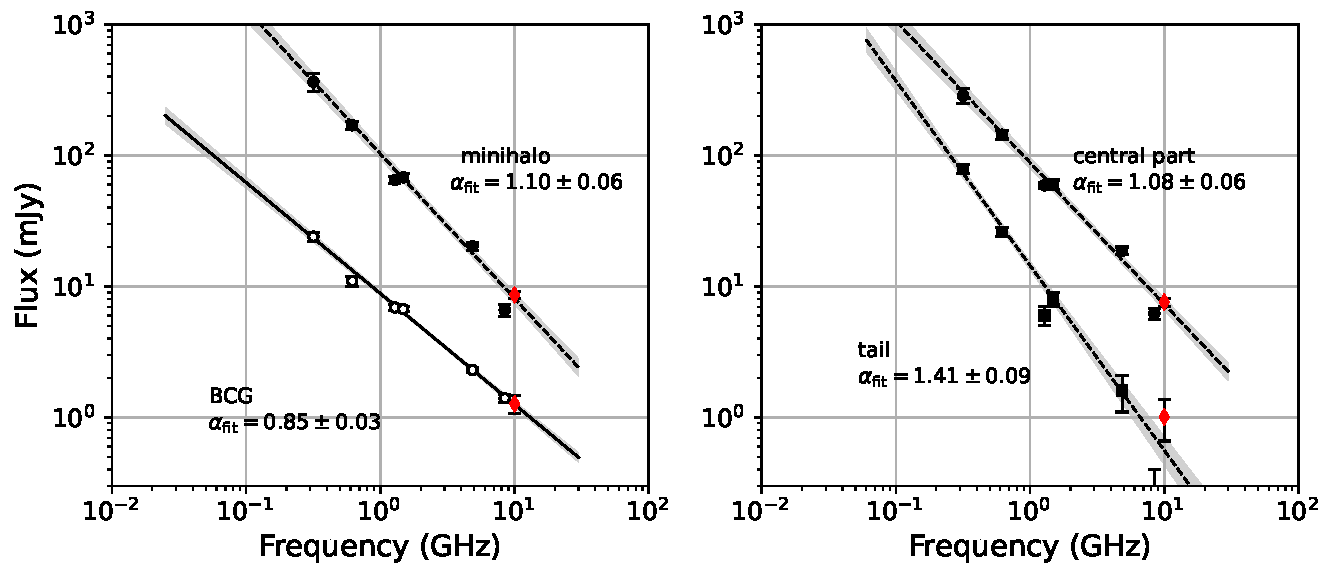
\includegraphics[width=\textwidth]{Chapter5/rxj1720_seds.pdf}
    \caption{RXJ1720+2368 radio spectra between 317 MHz and 10 GHz. \textit{Left Panel:} Spectrum of total minihalo (filled circles) and BCG (empty circles), red diamond denotes the 10 GHz measurement. The dotted line represents the minihalo power-law fit, solid line is BCG power-law spectrum, neither include the 8.44 GHz value. Grey shading as 1$\sigma$ error, slope and error are given in panel. \textit{Right Panel:} Spectrum of central (circles) and tail (squares) components. Dashed lines are are power-law fits over same range as left panel, grey shading indicates $1\sigma$ confidence, and slopes are reported.}
    \label{fig:rxj1720+2638_seds}
\end{figure}

\section{A478}

A478 is a nearby cool core cluster at a redshift of $z = 0.88$ \citep{Liu2024} . Chandra observations reveal a relaxed and highly elliptically symmetrical structure, with a central double-lobe BCG \citep{Sun2003, Bourdin2008}. The core temperature is $T \approx 1.54$ keV, increasing to $T\approx7.6$ keV at a radius of 260 kpc \citep{FanLam2024}. Two small ($\sim\!10$ kpc) X-ray cavities to the northeast and southwest are spatially aligned with the lobes of the BCG, indicating interaction between the BCG and ICM \citep{Sun2003}. A cold front is located 60 kpc to the southwest of the cluster \citep{Markevitch2003}. 

In the initial detection of minihalo emission, \citet{Giacintucci2014} note four several nearby radio sources to the minihalo. At 1.4 GHz, this includes the central BCG (S1), a head-tail to the east with a tail to the northwest (S4), a second head-tail within the tail of S4 with a tail to the northeast, and an unresolved source (S3) to the north of S2 and S4. The last source, S3, is likely to be a background source due to lacking optical correlations. \citet{Giacintucci2014} find the minihalo to be slightly extended more to the northeast ($R_{max} \sim 150$), compared to the other directions ($R_{min}\sim150$ kpc). This blends with the tail of S4, resulting in a large uncertainity in the flux estimate, due to difficulty in separating the tail and minihalo emission. They find the minihalo emission to be roughly constrained to the southwest cold front and a total flux $16.6\pm3$ mJy. LOFAR imaging at 144 MHz does not detect the diffuse minihalo emission, putting an upper bound on the spectral index of $\alpha < 1$ \citep{Savini2019}. Using archival GMRT data, \citet{Savini2019} finds S1 and S4 to have a spectral indices of $\sim\!1.1$ and $\sim\!0.6$, respectively, between 144 and 610 MHz. 

\subsection{10 GHz observation}
The observed minihalo region was much smaller than observed at 1.4 GHz, as to be expected. This resulted in only two contaminating sources, S1 and S4. The head-tail AGN doubled in brightness in the month between the D-configuration observations, causing severe PSF artefacts in the joint image. As such, this source was modelled on a per-dataset basis for the final self-calibration rounds. This variation was not observed in other point sources and could be attributed to a flare. The BCG exhibited time-variability within calibration error over all observations. The sources S2 and S3 are detected, but outside the radius of the observed minihalo. Three faint compact sources are located between S2 and the minihalo, but were spatially separate from the minihalo emission at the $3\sigma$ level. Point subtraction was then limited to S1 and S4 (including the tail) and used the standard 15 k$\lambda$ uv cut. The uv cut resulted in some emission remaining from S4, but as it was spatially distinct and the artefacts were successfully suppressed, this was left. The minihalo was modelled with scales $[0, 2, 4, 8, 16]$, \texttt{smallscalebias} of -0.5, and a \texttt{robust} of 1. The masking region was not clearly defined in \citep{Giacintucci2014}, so the mask used for flux estimation was determined by the $3\sigma$ region. 

The total minihalo flux was measured as $0.31 \pm 0.02$ mJy. The flux density of the BCG is $5.41 \pm 0.13$ mJy.

\begin{figure}
    \centering
    \includegraphics[width=0.85\textwidth]{Chapter5/vla_images/A478.pdf}
    \caption{RXJ1720+2638. Point source subtracted 10 GHz observation with restoring beam $5.55"\times4.96"$ at position angle -9.7\textdegree{} and noise $1\sigma = 1.88$ $\mu$Jy beam$^{-1}$. Contour levels (white) are spaced in factors of two starting from 3$\sigma$. The mask used for flux estimation is shown in by the dotted red line. The green cross marks the location of the subtracted BCG.}
    \label{fig:a478_image}
\end{figure}

\section{End}
Stick one big table of sources here? Ala Table 4 of G14 or Table 9 G19.

%CHAPTER 6
\chapter[Discussion]{Discussion}
\label{Chap:Discussion}

% \newcommand{\mhz}{\>\mathrm{MHz}}
% \newcommand{\ghz}{\>\mathrm{GHz}}

\section{Interpretation of results}
The interpretation of RXJ1720+2638 has previously been uncertain. An 8.44 GHz measurement suggested tentative evidence for steepening relative to lower frequencies \citep{Giacintucci2014a}, whereas \textit{uv}-plane modelling at 15.5 GHz was consistent with a single power-law spectrum \citep{Perrott2021}. The results of this thesis provide direct observational evidence in support of a single power-law spectrum up to at least 10 GHz. This is consistent with the conclusions of \citet{Perrott2021}, who argued that incomplete \textit{uv}-coverage at 8.44 GHz artificially reduced the measured flux density. 

The flux density measured over the tail region of the RXJ1720+2638 minihalo is approximately three times higher than that predicted by extrapolation of previous measurements. One possible explanation is the use of a different spatial mask, which may include a larger fraction of the brighter central emission within the region classified as the tail. As the mask was estimated by eye from the previous studies, this is plausible. The detectable high-frequency emission extends over only approximately half of the masked tail region. This reduction in spatial extent with increasing frequency is consistent with a steepening spectral index along the tail, as radiative losses progressively suppress the population of high-energy electrons. The results for this cluster will be explored in more depth in a forthcoming study (Colquhoun et al., in prep). 

The findings for RXCJ1115+0129 are somewhat less constraining, primarily due to the limited number of flux density measurements for this minihalo. The previous study by \citet{Trehaeven2023} found a spectral index of $\alpha=1.0\pm1.1$ between 1--1.5 GHz, with the uncertainty dominated by subtraction errors. The results presented in this thesis are consistent with their mean value and reduce the uncertainty by approximately a factor of six, although the uncertainty remains dominated by source subtraction. The northern and southern spatial steepening reported in the previous study was not explored in depth in this thesis. However, the narrower observed spatial extent at 10 GHz is near-aligned with the direction of their measured steepening. A spatially resolved point-to-point analysis combining the 1.3 GHz MeerKAT data with the 10 GHz observations presented here would provide a more robust test for this feature.

Several previous flux density measurements for the RXJ2129+0005 minihalo were available for comparison with the value measured in this thesis. The 10 GHz flux density is found to be slightly higher than expected from the extrapolation of the previous studies, although the $1\sigma$ uncertainties overlap. The excess flux may arise from two regions of emission near the masking boundary, including the unsubtracted source S2 and a diffuse region to the east (see Figure \ref{fig:rxj2129_sub_image}). These may contaminate the masked area and introduce flux not associated with the minihalo. The complex masking region defined by \citet{Giacintucci2014} was approximated here by an ellipse, which further modifies the measured flux density. Notably, the flux density measured within the $3\sigma$ contour is less than half that of the larger mask ($S_{3\sigma} = 0.15\pm0.1$ mJy compared to $S_{mask} = 0.41\pm0.1$ mJy), which demonstrates the sensitivity of the integrated flux to the adopted mask.

The final cluster measured in this thesis, A478, presents a more intriguing case. Previous studies placed only an upper limit on the spectral index of $\alpha<1$, whereas the flux density measured in this thesis implies a far greater spectral index of $\alpha = 2.02\pm0.10$. The in-band spectral index is even steeper at $\alpha = 3.34\pm0.18$, suggesting significant spectral curvature between 1.4 and 10 GHz. This result should be interpreted with caution, however, as it is based upon only two direct measurements and one non-detection. The adopted mask and \textit{uv}-range likely differ from those used by \citet{Giacintucci2014} and \citet{Savini2019}. Spatial filtering at 10 GHz may result in missing flux, analagous to the 8.44 GHz measurement of RXJ1720+2638. Additional intermediate-frequency observations (e.g. 144 MHz to 5 GHz) are required to determine whether this apparent steepening reflects genuine particle ageing or residual systematic effects. Nevertheless, A478 remains an outlier compared to the other clusters in this sample.

The clusters RXJ1720+2638, RXCJ1115+0129, and RXJ2129+0005 exhibit total 10 GHz flux densities consistent, within uncertainties, with the extrapolated power-law spectra derived from lower-frequency measurements. The absence of clear high-frequency curvature in the integrated spectra suggests that strong radiative ageing effects are not dominant over this frequency range. This behaviour is broadly consistent with the expectations from the hadronic scenario, in which secondary electrons are continuously injected and maintain a single power-law energy distribution to high frequencies.

In contrast, the turbulent acceleration models predict spectral steepening at high-frequencies once the stochastic acceleration becomes inefficient at compensating for radiative losses of the CRe population. The results presented here therefore suggest that turbulent reacceleration, if present, is not dominant at the minihalo scale or that an additional mechanism is sustaining the high-energy CRe population. However, the spatially resolved steepening observed in the tail of RXJ1720+2638, together with the tentative evidence of curvature in A478, indicates that multiple mechanisms may operate within individual clusters. This interpretation is consistent with previous studies (e.g \citealp{Perrott2021, Riseley2024}).

\section{Incomplete clusters}
For the majority of the remaining clusters in this sample a minihalo is detected at 10 GHz. However, difficulties encountered during the subtraction of contaminating emission prevented robust estimation of the minihalo flux in several cases. These difficulties can be categorised as arising from (i) variability of compact sources between observing epochs and (ii) residual diffuse emission not associated with the minihalo in the subtracted image. 

Variability of compact sources between observations at different epochs presents a significant challenge for the self-calibration and source subtraction. Point source modelling was performed independently for each dataset in order to mitigate this effect. However, this did not fully resolve the residual artefacts in the individual models nor the joint image. The C-configuration observations were typically the dominant contributor to subtraction errors in the combined datasets image, although the precise reason behind this remains unclear. Possible factors are the \texttt{tclean} parameters for imaging of the point sources and residual calibration errors.

The clusters where a minihalo was not detected at 10 GHz are A1795 and A2626. In both cases, the absence of a clear detection is attributed to imaging artefacts obscuring potential diffuse emission, rather than insufficient surface brightness sensitivity. These clusters contain bright central AGNs that complicated the self-calibration process. It is plausible that with additional refinement of the self-calibration process, a reliable image of the minihalo emission could be recovered. 

The models used for source subtraction were constructed using a fixed \textit{uv}-cut and imaging parameters derived from an analysis of a single cluster, RXJ1720+2638 (see Section \ref{sec:source_subtraction}). Although manual inspection of each resulting image was performed, these parameters likely require optimisation on a per-cluster basis. A key systematic limitation arises because the adopted \textit{uv}-cut corresponds to a constant angular scale on the sky, rather than a constant physical scale.

The clusters in this sample span physical scales between 0.72 and 7.5 kpc arcsec$^{-1}$, increasing with redshift under the adopted cosmology. Consequently, the same angular \textit{uv}-cut corresponds to substantially different physical scales across the sample. RXJ1720+2638 lies at an intermediate redshift within the cluster sample. For lower-redshift clusters an identical \textit{uv}-cut selects smaller physical scales. In such cases, diffuse emission from AGN lobes may not be fully included in the subtraction model, leading to residual contamination in the subtracted image (e.g. 2A0335+096). 

Conversely, for higher-redshift clusters, the same \textit{uv}-cut corresponds to larger physical scales. This increase the risk that extended minihalo emission is partially incorporated into the subtraction model, resulting in over-estimation of compact source flux densities, and subsequently, over-subtraction in the final image (e.g ACTJ0022-0036). 

The impact of adopting a constant angular \textit{uv}-cut is dependent on the minihalo extent, cluster redshift, and the morphology of embedded radio sources. A physically motivated \textit{uv}-cut scaled to the observed extent may reduce this systematic bias in future analyses.

\section{Measurement Limitations}
There are several fundamental observational limitations affecting the detectability of minihalos in this study. The primary constraints arise from the maximum recoverable scale, surface brightness sensitivity, and angular resolution of the interferometer configuration. 

\subsection{Maximum recoverable scale}
The largest angular scale that the interferometer can recover is set by the minimum projected baseline length. For these VLA observations, the shortest baselines correspond to 1 k$\lambda$. Approximating the angular scale as $\theta \approx 1/\vec u$ yields $10^{-3}$ rad or $\sim\!3.44$ arcminutes. 

For a characteristic minihalo diameter of $\sim\!300$ kpc, this angular scale corresponds to a minihalo located at redshift $z \sim 0.07$. Below this redshift, emission at scales comparable to or larger than this minihalo diameter may be partially resolved out, leading to an underestimation of the total flux density. 

This effect is most relevant for three clusters in this sample, 2A0335+096, A2626, and A1795. Of these clusters, only 2A0335+096 has a source-subtracted image. For this cluster $3.44'$ corresponds to $\approx150$ kpc. Diffuse emission extending beyond this scale will not be fully recovered. However, the lowest-redshift cluster for which a total 10 GHz flux density was successfully measured is RXJ1720+2638 at $z=2.775$. This corresponds to a maximum physical scale of $\sim\!570$ kpc, suggesting that spatial filtering is unlikely to significantly bias the integrated flux densities reported here. Matching the \textit{uv}-coverage with prior studies, as performed for RXJ1720+2638, also ensures any spatial filtering is consistent between studies.

\subsection{Surface brightness sensitivity}

The surface brightness sensitivity is limited by image noise, which arises from residual RFI, calibration uncertainties, and instrumental thermal noise. For the 10 GHz observations presented here, the typical rms noise level is approximately $3$ $\mu$Jy beam$^{-1}$. 

For steep-spectrum or intrinsically low-brightness minihalos, emission may fall below the adopted $3\sigma$ detection threshold. This can artifically reduce the apparent spatial extent of the emission relative to lower-frequency observations, where surface brightness is higher. In such cases, only lower limits on the spectral index can be derived. As discussed previously, spatial masks defined in earlier studies were adopted where available to ensure consistency in flux density measurements. 

One method to increase the signal-to-noise ratio of diffuse emission is to smooth an image, typically by convolution with a Gaussian kernel. Such spatial averaging enhances low-surface brightness emission but reduces spatial resolution. This process disproportionally affects compact sources relative to extended emission, as their flux is redistributed over a larger area. Consequently, smoothing is more appropriately applied to source-subtracted images. This approach was not explored in this thesis and remains a potential avenue for future refinement of these measurements.

\subsection{Angular resolution}
The angular resolution, defined by the restoring beam, has the greatest impact on the accuracy of the source subtraction. For the 10 GHz observations, the typical restoring beam is approximately $4"\times3"$. Higher angular resolution improves the modelling of compact sources and their associated lobes or jets, enabling more effective separation from the diffuse minihalo emission.

Many compact sources are unresolved at this beam size. Improved resolution allows subtraction to occur over smaller areas, thereby reducing subtraction uncertainties. Since the subtraction error scales with the area over which the model is removed, $\sigma_{sub} \propto A_{sub}$, improved resolution directly reduces residual contamination. As discussed previously, the inclusion of C-configuration data provides the necessary angular resolution in the joint imaging process.

\section{SZ effect}
The SZ effect represents a potential contaminant to the flux densities measured in this thesis. As it arises from IC-scattering through the cluster, it is naturally a cluster-scale phenomenon extending well beyond the spatial extent of the minihalo. Such a large-scale structure may be partially sampled at the shortest baselines of the 10 GHz observations. 

The thermal SZ spectrum has a null frequency at 217 GHz, where there is no contribution. Below this frequency the effect is negative, suppressing the measured flux density, while above it the effect is positive. At 10 GHz the effect is therefore negative. However, the amplitude of the SZ decrement is expected to be small. Figure \ref{fig:sz_amp} depicts example spectra for the SZ effect.

\begin{figure}
    
\includegraphics[width=0.85\textwidth]{Chapter6/sz_ampl.pdf}
    \caption{Thermal SZ intensity spectrum illustrating characteristic frequency dependence. Curves correspond to representative Compton-$y$ values, with larger $y$ typically associated with more massive clusters. The dotted black line denotes the null frequency at 217 GHz.}
    \label{fig:sz_amp}
\end{figure}


\citet{Perrott2021} estimated the maximum SZ signal for RXJ1720+2638 for the VLA observation at 8.44 GHz. They found a negative maximum amplitude of approximately 80 $\mu$Jy at the shortest baselines. Given the similar observing frequency and comparable interferometer configuration, this provides a reasonable estimate for the expected SZ signal. For RXJ1720+2638 this is negligible compared to the measured minihalo flux and lies well within the quoted uncertainty.

The remaining clusters where minihalo fluxes are obtained (A478, RXCJ1115+0129, and RXJ2129+0005) have masses within $-26\%$ to $+18\%$ of RXJ1720+2638. As the SZ effect scales primarily with the integrated thermal pressure (and therefore cluster mass), a very conservative upper bound of $<0.1$ mJy is considered for all clusters. This is within the measurement uncertainties for RXCJ1115+0129 and RXJ2129+0005. For A478, this represents approximately 33\% of the measured flux. However, this difference is insufficient to reconcile the order of magnitude discrepancy to the lower limit on the spectral index reported by \citet{Savini2019}.

Given that the SZ contribution is comparable to or below the measurement uncertainties, it is unlikely to significantly affect the conclusions presented here. A more rigorous treatment would involve modelling the SZ signal for each cluster using gas pressure profiles and propagating through the interferometer response, as performed by \citet{Perrott2021}. Such analysis is beyond the scope of this thesis, but would enable the direct correction of the minihalo flux densities.


%CONCLUSION CHAPTER
% ***************************************************
% Conclusion
% ***************************************************
\chapter[Conclusion]{Conclusion}
\label{Chap:Conclusion}

The aim of this thesis was to investigate the production mechanisms behind the diffuse emission of minihalos. A key observational distinction between hadronic production and turbulent reacceleration lies in the high-frequency spectral steepening predicted by the reacceleration scenario. To investigate this, radio observations at 10 GHz for a sample of twelve galaxy cluster minihalos were analysed during this thesis. The results indicate that high-frequency spectral steepening $<10$ GHz is not common among minihalos for which robust flux measurements were obtained.

These datasets were calibrated and jointly imaged to combine the higher angular resolution of C-configuration observations with the better sensitivity to extended emission of D-configuration data. A custom calibration stage was implemented to improve the removal of radio-frequency interference within the observations. The resulting images were source-subtracted to isolate the diffuse emission of the minihalo, and subsequently utilised to calculate the total flux density. This was successfully completed for four clusters, RXJ1720+2638, A478, RXCJ1115+0129, and RXJ2129+0005. The majority of the remaining clusters displayed evidence of a minihalo, however, imaging artefacts prevented a reliable measurement of the total minihalo emission.

The resulting flux densities were compared to previous studies and used to calculate the spectral indices for each minihalo. Three of these clusters (RXJ1720+2638, RXCJ1115+0129, RXJ2129+0005) are consistent with a single power-law up to 10 GHz, with spectral indices in the range $\alpha\approx1$--1.1. One cluster (A478) exhibits potential steepening, with a derived spectral index of $\alpha=2.02$, compared to the lower frequency upper bound of $\alpha\leq1$. The single power-law spectrum is broadly consistent with the hadronic scenario, while the steepening is more consistent with the turbulent reacceleration method. These results suggest that both mechanisms can operate within the minihalo, with hadronic production potentially playing a dominant role in many systems. 

The measured spectral indices can be biased by the defined spatial mask, \textit{uv}-coverage, and source-subtraction between observations at different frequencies. Differences in masking strategies and \textit{uv}-coverage between studies makes comparison to the results here more ambiguous, as spatial filtering from mismatched coverages can artificially reduce the measured flux. Furthermore, the sample size for measured flux densities limits a statistical inference on the general behaviour of minihalos. The final uncertainties for the flux densities measured for this thesis are dominated by the source-subtraction component, particularly for low surface-brightness minihalos.

A first step can be achieved by completing the self-calibration and source-subtraction for the calibrated datasets in this sample. This would enable a broader spectral comparison between the clusters. An exploration of the spatial dependence of the spectral index would also assist in distinguishing between the hadronic scenario and turbulent reacceleration. A spatial investigation comparing to lower frequency observations may reveal if these mechanisms operate over different minihalo regions, as previously observed for RXJ1720+2638. 

The findings of this thesis extend high-frequency constraints on minihalo spectra. The absence of widespread spectral steepening challenges simple reacceleration-only models. These observations constitute the first high-frequency survey of radio minihalos, highlighting the importance of multi-frequency and spatially resolved studies. 

% ***************************************************
% Bibliography
%****************************************************
%CHOOSE YOUR BIB STYLE AND FILE.
%We have included the following two referencing styles for you to use in your thesis. You can add an alternate style if you prefer.

%Style: apalike = this is an (Author, Year) referencing style similar to APA
%Style: elsarticle-num = this is a numbered referencing style that will display the bibliography in citation order

%To use one of the styles provided ensure the % is removed from the start of the line, and the other option is commented out with a % at the start of the line. The style elsarticle-num is active by default.

\bibliographystyle{apalike}
% \bibliographystyle{elsarticle-num}

\bibliography{./References/Bibliography}

%When you have finished your thesis we recommend that you manually fix any errors in your bibliography. 
%To do this, compile, copy the .bbl into a new .tex file and include this here after commenting out the other bibliography commands. Make corrections in that .tex file.

% ***************************************************
% Appendices
%**************************************************** 
%UNCOMMENT THIS SECTION IF YOU ARE USING APPENDICES.
%Simply adapt the same formatting used for other chapters.
% \appendix
% % If you need appendix in your thesis then consider the following appendix file (you can add more if you need more) otherwise you should not consider it in your main thesis.
% % ***************************************************
% Appendix
% ***************************************************

\chapter{Example \texttt{AOFLAGGER} Lua script}
\label{app:aoflagger}
The \texttt{AOFLAGGER} strategy used for the flagging of RFI in this thesis consists of two targeted passes, and a final general pass, designed to address the different RFI environments present across the full 8--12 GHz frequency band. An example of the script is provided in this appendix, the complete scripts used during the calibration process are available in the associated GitHub repository under `Data Processing' and the relevant observation ID.\footnote{\url{https://github.com/MoonlitMoo/Masters-2025}}

The \texttt{options} function defines the spectral windows that are flagged by each pass, and the corresponding execution function. The first pass (\texttt{execute\_awr}) targets spectral windows 10--11, corresponding to frequencies $\approx$9.3--9.5 GHz which contain intermittent satellite RFI. The second pass (\texttt{execute\_microwave}) covers spectral windows 22--31 (approximately 10.7--12 GHz), where continuous ground-based communication interference is present. The final pass (\texttt{execute\_final}) applies to the full frequency band 8--12 GHz. The targeted passes use independent lower flagging thresholds than the final pass, providing adaptability to the amount of RFI measured in an observation. The values shown are representative of those used in the calibration process, with thresholds ranging from 0.65 to 5.0.

\begin{lstlisting}[
    language=Lua, 
    caption={Example \texttt{AOFLAGGER} Lua script.}, 
    label={lst:reduction},
    literate={é}{{\'e}}1, 
    numberstyle=\tiny,
    basicstyle=\ttfamily\footnotesize
]
aoflagger.require_min_version("3.0")

function options()
  opts1 = {
    ["bands"] = {10,11},
    ["execute-function"] = "execute_awr",

  }

  opts2 = {
    ["bands"] = {22,23,24,25,26,27,28,29,30,31},
    ["execute-function"] = "execute_microwave"
  }

  opts3 = {
    ["execute-function"] = "execute_final"
  }

  return {
    ["1 - weather radars"] = opts1,
    ["2 - microwave link"] = opts2,
    ["3 - final sweep"] = opts3
  }
end

function execute_awr(input)
    -- 9.3-9.5 GHz (airborne weather radars)
    trim_rfi(input, 1.0, 1.0)
end

function execute_microwave(input)
    -- 10.7-12 GHz (Microwave link + geostationary satellite near 11.7-12 GHz)
    trim_rfi(input, 1.0, 1.0)
end

function execute_final(input)
    -- Run over remaining at the end as cleanup
    trim_rfi(input, 2.0, 2.0)
end

function trim_rfi(input, base_threshold, transient_threshold_factor)
  -- base_threshold, lower means more sensitive detection
  -- transient_threshold_factor, decreasing this value makes detection of transient RFI more aggressive
  local flag_polarizations = input:get_polarizations()
  local flag_representations = { "amplitude" }
  local iteration_count = 4 -- how many iterations to perform?
  local threshold_factor_step = 1.75 -- How much to increase the sensitivity each iteration?
  local exclude_original_flags = true
  local frequency_resize_factor = 1.0 -- Amount of "extra" smoothing in frequency direction

  local inpPolarizations = input:get_polarizations()

  if not exclude_original_flags then
    input:clear_mask()
  end
  local copy_of_input = input:copy()

  for ipol, polarization in ipairs(flag_polarizations) do
    local pol_data = input:convert_to_polarization(polarization)
    local converted_data
    local converted_copy

    for _, representation in ipairs(flag_representations) do
      converted_data = pol_data:convert_to_complex(representation)
      converted_copy = converted_data:copy()

      for i = 1, iteration_count - 1 do
        local threshold_factor = threshold_factor_step ^ (iteration_count - i)

        local sumthr_level = threshold_factor * base_threshold
        if exclude_original_flags then
          aoflagger.sumthreshold_masked(
            converted_data,
            converted_copy,
            sumthr_level,
            sumthr_level * transient_threshold_factor,
            true,
            true
          )
        else
          aoflagger.sumthreshold(converted_data, sumthr_level, sumthr_level * transient_threshold_factor, true, true)
        end

        -- Do timestep & channel flagging
        local chdata = converted_data:copy()
        aoflagger.threshold_timestep_rms(converted_data, 2.0)
        aoflagger.threshold_channel_rms(chdata, 1.5 * threshold_factor, true)
        converted_data:join_mask(chdata)

        -- High pass filtering steps
        converted_data:set_visibilities(converted_copy)
        if exclude_original_flags then
          converted_data:join_mask(converted_copy)
        end

        local resized_data = aoflagger.downsample(converted_data, 3, frequency_resize_factor, true)
        aoflagger.low_pass_filter(resized_data, 21, 31, 2.5, 5.0)
        aoflagger.upsample(resized_data, converted_data, 3, frequency_resize_factor)

        local tmp = converted_copy - converted_data
        tmp:set_mask(converted_data)
        converted_data = tmp

        aoflagger.visualize(converted_data, "Residual #" .. i, i + iteration_count)
        aoflagger.set_progress((ipol - 1) * iteration_count + i, #flag_polarizations * iteration_count)
      end -- end of iterations

      if exclude_original_flags then
        aoflagger.sumthreshold_masked(
          converted_data,
          converted_copy,
          base_threshold,
          base_threshold * transient_threshold_factor,
          true,
          true
        )
      else
        aoflagger.sumthreshold(converted_data, base_threshold, base_threshold * transient_threshold_factor, true, true)
      end
    end -- end of complex representation iteration

    if exclude_original_flags then
      converted_data:join_mask(converted_copy)
    end

    -- Helper function used below
    function contains(arr, val)
      for _, v in ipairs(arr) do
        if v == val then
          return true
        end
      end
      return false
    end

    if contains(inpPolarizations, polarization) then
      if input:is_complex() then
        converted_data = converted_data:convert_to_complex("complex")
      end
      input:set_polarization_data(polarization, converted_data)
    else
      input:join_mask(converted_data)
    end

    aoflagger.visualize(converted_data, "Residual #" .. iteration_count, 2 * iteration_count)
    aoflagger.set_progress(ipol, #flag_polarizations)
  end -- end of polarization iterations

  if exclude_original_flags then
    aoflagger.scale_invariant_rank_operator_masked(input, copy_of_input, 0.2, 0.2)
  else
    aoflagger.scale_invariant_rank_operator(input, 0.2, 0.2)
  end

  aoflagger.threshold_timestep_rms(input, 4.0)

  input:flag_nans()
end
\end{lstlisting}


\end{document}
